\documentclass[man]{apa6}
\usepackage{lmodern}
\usepackage{amssymb,amsmath}
\usepackage{ifxetex,ifluatex}
\usepackage{fixltx2e} % provides \textsubscript
\ifnum 0\ifxetex 1\fi\ifluatex 1\fi=0 % if pdftex
  \usepackage[T1]{fontenc}
  \usepackage[utf8]{inputenc}
\else % if luatex or xelatex
  \ifxetex
    \usepackage{mathspec}
  \else
    \usepackage{fontspec}
  \fi
  \defaultfontfeatures{Ligatures=TeX,Scale=MatchLowercase}
\fi
% use upquote if available, for straight quotes in verbatim environments
\IfFileExists{upquote.sty}{\usepackage{upquote}}{}
% use microtype if available
\IfFileExists{microtype.sty}{%
\usepackage{microtype}
\UseMicrotypeSet[protrusion]{basicmath} % disable protrusion for tt fonts
}{}
\usepackage{hyperref}
\hypersetup{unicode=true,
            pdftitle={The development of infants' responses to mispronunciations - A Meta-Analysis},
            pdfauthor={Katie Von Holzen~\& Christina Bergmann},
            pdfkeywords={keywords},
            pdfborder={0 0 0},
            breaklinks=true}
\urlstyle{same}  % don't use monospace font for urls
\usepackage{graphicx,grffile}
\makeatletter
\def\maxwidth{\ifdim\Gin@nat@width>\linewidth\linewidth\else\Gin@nat@width\fi}
\def\maxheight{\ifdim\Gin@nat@height>\textheight\textheight\else\Gin@nat@height\fi}
\makeatother
% Scale images if necessary, so that they will not overflow the page
% margins by default, and it is still possible to overwrite the defaults
% using explicit options in \includegraphics[width, height, ...]{}
\setkeys{Gin}{width=\maxwidth,height=\maxheight,keepaspectratio}
\IfFileExists{parskip.sty}{%
\usepackage{parskip}
}{% else
\setlength{\parindent}{0pt}
\setlength{\parskip}{6pt plus 2pt minus 1pt}
}
\setlength{\emergencystretch}{3em}  % prevent overfull lines
\providecommand{\tightlist}{%
  \setlength{\itemsep}{0pt}\setlength{\parskip}{0pt}}
\setcounter{secnumdepth}{0}
% Redefines (sub)paragraphs to behave more like sections
\ifx\paragraph\undefined\else
\let\oldparagraph\paragraph
\renewcommand{\paragraph}[1]{\oldparagraph{#1}\mbox{}}
\fi
\ifx\subparagraph\undefined\else
\let\oldsubparagraph\subparagraph
\renewcommand{\subparagraph}[1]{\oldsubparagraph{#1}\mbox{}}
\fi

%%% Use protect on footnotes to avoid problems with footnotes in titles
\let\rmarkdownfootnote\footnote%
\def\footnote{\protect\rmarkdownfootnote}


  \title{The development of infants' responses to mispronunciations - A
Meta-Analysis}
    \author{Katie Von Holzen\textsuperscript{1,2}~\& Christina
Bergmann\textsuperscript{3,4}}
    \date{}
  
\shorttitle{Mispronunciation Meta-Analysis}
\affiliation{
\vspace{0.5cm}
\textsuperscript{1} Department of Hearing and Speech Sciences, University of Maryland, USA\\\textsuperscript{2} Laboratoire Psychologie de la Perception, Université Paris Descartes\\\textsuperscript{3} Max Planck Institute for Psycholinguistics, Nijmegen, the Netherlands\\\textsuperscript{4} LSCP, Departement d'Etudes Cognitives, ENS, EHESS, CNRS, PSL Research University}
\keywords{keywords\newline\indent Word count: X}
\usepackage{csquotes}
\usepackage{upgreek}
\captionsetup{font=singlespacing,justification=justified}

\usepackage{longtable}
\usepackage{lscape}
\usepackage{multirow}
\usepackage{tabularx}
\usepackage[flushleft]{threeparttable}
\usepackage{threeparttablex}

\newenvironment{lltable}{\begin{landscape}\begin{center}\begin{ThreePartTable}}{\end{ThreePartTable}\end{center}\end{landscape}}

\makeatletter
\newcommand\LastLTentrywidth{1em}
\newlength\longtablewidth
\setlength{\longtablewidth}{1in}
\newcommand{\getlongtablewidth}{\begingroup \ifcsname LT@\roman{LT@tables}\endcsname \global\longtablewidth=0pt \renewcommand{\LT@entry}[2]{\global\advance\longtablewidth by ##2\relax\gdef\LastLTentrywidth{##2}}\@nameuse{LT@\roman{LT@tables}} \fi \endgroup}


\DeclareDelayedFloatFlavor{ThreePartTable}{table}
\DeclareDelayedFloatFlavor{lltable}{table}
\DeclareDelayedFloatFlavor*{longtable}{table}
\makeatletter
\renewcommand{\efloat@iwrite}[1]{\immediate\expandafter\protected@write\csname efloat@post#1\endcsname{}}
\makeatother
\usepackage{lineno}

\linenumbers
\usepackage{setspace}
\AtBeginEnvironment{tabular}{\singlespacing}
\AtBeginEnvironment{lltable}{\singlespacing}
\AtBeginEnvironment{tablenotes}{\doublespacing}
\captionsetup[table]{font={stretch=1.5}}
\captionsetup[figure]{font={stretch=1.5}}

\authornote{

Correspondence concerning this article should be addressed to Katie Von
Holzen, 0221A LeFrak Hall, University of Maryland, College Park, MD
20742. E-mail:
\href{mailto:katie.m.vonholzen@gmail.com}{\nolinkurl{katie.m.vonholzen@gmail.com}}}

\abstract{
One or two sentences providing a \textbf{basic introduction} to the
field, comprehensible to a scientist in any discipline.

Two to three sentences of \textbf{more detailed background},
comprehensible to scientists in related disciplines.

One sentence clearly stating the \textbf{general problem} being
addressed by this particular study.

One sentence summarizing the main result (with the words ``\textbf{here
we show}'' or their equivalent).

Two or three sentences explaining what the \textbf{main result} reveals
in direct comparison to what was thought to be the case previously, or
how the main result adds to previous knowledge.

One or two sentences to put the results into a more \textbf{general
context}.

Two or three sentences to provide a \textbf{broader perspective},
readily comprehensible to a scientist in any discipline.


}

\usepackage{amsthm}
\newtheorem{theorem}{Theorem}[section]
\newtheorem{lemma}{Lemma}[section]
\theoremstyle{definition}
\newtheorem{definition}{Definition}[section]
\newtheorem{corollary}{Corollary}[section]
\newtheorem{proposition}{Proposition}[section]
\theoremstyle{definition}
\newtheorem{example}{Example}[section]
\theoremstyle{definition}
\newtheorem{exercise}{Exercise}[section]
\theoremstyle{remark}
\newtheorem*{remark}{Remark}
\newtheorem*{solution}{Solution}
\begin{document}
\maketitle

\section{Introduction}\label{introduction}

Acquiring a first language means that young learners are solving a host
of tasks in a short amount of time. As infants develop into toddlers
during their second and third years they learn new words in earnest
while simultaneously refining their knowledge about the sounds that make
up these words {[}Primir, Kuhl, Best{]}. In a mature phono-lexical
system, word recognition must balance flexibility to slight variation
(e.g., speaker identity, accented speech) while distinguishing between
phonetic details that differentiate words in their native language
(e.g.~cat-hat). To build robust language knowledge, it seems ueful to
acquire this ability early during development. Indeed, before children
can correctly pronounce a word, they already are aware that slight
phonological deviations might signal a change in word meaning {[}Clark
\& Clark, 1977{]}. This mispronunciation sensitivity reflects the
specificity with which infants represent the phonological information of
familiar words. As infants continue to develop into expert language
users, their language processing matures and becomes more efficient,
including their knowledge of what consistutes a permissible versus
word-changing phonological deviation. In this paper, we aggregate and
analyze the almost 20 years of literature investigating mispronunciation
sensitivity in infants in an attempt to uncover its characteristics and
the trajectory of its development.

At the turn of the millenia, infant language acquisition researchers had
established that during their first years of life, infants are sensitive
to changes in the phonetic detail of newly segmented words (Jusczyk \&
Aslin, 1995) and learned minimal pairs (Stager \& Werker, 1997).
Furthermore, when presented with familiar image pairs, children fixate
on one image upon hearing its label (Fernald, Pinto, Swingley, Weinberg,
\& McRoberts, 1998; Tincoff \& Jusczyk, 1999). Swingley and Aslin (2000)
were the first to tie these lines of research together and investigate
mispronunciation sensitivity in infant familiar word recognition:
Children aged 18 to 23 months learning American English saw pairs of
images (e.g.~a baby and a dog) and their eye movements to each image
were recorded and subsequently coded offline. On \enquote{correct}
trials, children heard the correct label for one of the images (e.g.
\enquote{baby}). On \enquote{mispronounced} trials, children heard a
mispronounced label of one of the images (e.g. \enquote{vaby}). The mean
proportion of fixations to the target image (here: a baby) was
calculated separately for both correct and mispronounced trials by
dividing the target looking time by the sum of total looking time to
both target and a distractor (proportion of target looking or PTL). Mean
fixations in correct trials were significantly greater than in
mispronounced trials, and in both conditions looks to the target were
significantly greater than chance. We refer to this pattern of a
difference between looks to correct and mispronounced words as
\emph{mispronunciation sensitivity} and of looks to the target image
above chance in each condition as \emph{object identification}. Swingley
and Aslin (2000) concluded that already before the second birthday,
children represent words with sufficient detail to be sensitive to
mispronunciations.

The study of Swingley and Aslin (2000) as well as subsequent studies
examining mispronunciation sensitivity address two complementary
principles that infants must discover in early phonological development
in order to form adult-like word representations: \emph{phonological
constancy} and \emph{phonological distinctiveness}. Phonological
constancy is the ability to resolve phonological variation across
different instances of a word, as long as the variation does not
compromise the overall identity of the word. For example, different
speakers - particularly across genders and accents - produce the same
word with notable acoustic variation, although the word remains the
same. In contrast, phonological distinctiveness describes the ability to
differentiate between different words that happen to be phonologically
similar, such as bad/bed or cat/hat. To successfully recognize words,
speakers of a given language must therefore simultaneously use both
phonological constancy and distinctiveness to determine where
phonological variation is appropriate and where it changes a word's
meaning. Both abilities have to be acquired, because language systems
differ in which sounds signal a meaning change.

{[}Katie: since we actually don't have theoretical framework support for
the no-change theory, I've changed around the sentence below to
explicitly say that only 2 of the 3 are predicted by theoretical
accounts.{]}{[}Christina: Works for me. I am just thinking what the
Vihman-style framework says. do you happen to know? I think the Renner
thesis discusses it.{]} {[}Katie: I wasn't really familiar with the
Vihman framework, but looking at Renner's thesis and some of the
original papers suggests that it really is about production, not
perception.{]}

In the current study, we focus on infants' developing ability to
correctly apply the principles of phonological distinctiveness and
constancy by using a meta-analytic approach to investigate
mispronunciation sensitivity. Considering that infants are sensitive to
mispronunciations and that, in general, their processing matures with
development, we examine the shape of mispronunciation sensitivity over
the course of the second and third year. There are three distinct
possibilities how mispronunciation sensitivity might change as infants
become native speakers, which are all respectively supported by single
studies and two predicted by theoretical accounts. By aggregating all
publicly available evidence using meta-analysis, we can examine
developmental trends making use of data from a much larger and diverse
sample of infants than is possible in most single studies (see Frank et
al., 2018; for a notable exception). Before we outline the
meta-analytical approach and its advantages in detail, we first discuss
the proposals this study seeks to disentangle and the data supporting
each of the accounts.

Young infants may begin cautiously in their approach to word
recognition, rejecting any phonological variation in familiar words and
only later learning to accept appropriate variability. According to the
Perceptual Attunement account, this describes a shift away from specific
native phonetic patterns to a more mature understanding of the abstract
phonological structure of words (Best 1994, 1995). This shift is
predicted to coincide with the vocabulary spurt around 18 months, and is
therefore related to vocabulary growth. In this case, we would expect
the size of mispronunciation sensitivity to be larger at younger ages
and \emph{decrease} as the child matures and learn more words, although
children continue to detect mispronunciations. Indeed, young infants are
more perturbed by accented speakers than older infants in their
recognition of familiar words (Best, Tyler, Gooding, Orlando, \& Quann,
2009; Mulak, Best, \& Tyler, 2013) or learning of new words (Schmale,
Hollich, \& Seidl, 2011).

According to a different theoretical framework, young infants may
instead begin with phonologically broad representations for familiar
words and only refine their representations as language experience
accumulates. PRIMIR (Processing Rich Information from Multidimensional
Interactive Representations; Curtin \& Werker, 2007; Werker \& Curtin,
2005; Curtin, Byers-Heinlein, \& Werker, 2011) describes the development
of phonemic categories emerging as the number of word form-meaning
linkages increases. Vocabulary growth, therefore, promotes more detailed
phonological representations in familiar words. Following this account,
we predict an \emph{increase} in mispronunciation sensitivity as infants
mature and add more words to their growing lexicon.

Finally, sensitivity to mispronunciation may not be modulated by
development at all. Infants' overall language processing becomes more
efficient, but their sensitivity to mispronunciations may not change.
Across infancy and toddlerhood, mispronunciations would thus be detected
and lead to less looks at a target than correct pronunciations, but the
size of this effect would not change, nor be related to vocabulary size.
This pattern is not predicted by any mainstream theory of language
acquisition, but for completeness we mention it here.

Research following the seminal study by Swingley and Aslin (2000) has
extended mispronunciation sensitivity to infants as young as 9 months
(Bergelson \& Swingley, 2017), indicating that from early stages of the
developing lexicon onwards, infants can and do detect mispronunciations.
Regarding the change in mispronunciation sensitivity over development,
however, only a handful of studies have compared more than one age group
on the same mispronunciation task (see Table X), making the current
meta-analysis very informative. One study has found evidence for infants
to become \emph{less} sensitive to mispronunciations as children
develop. Mani and Plunkett (2011) presented 18- and 24-month-olds with
mispronunciations varying in the number of features changed (see below
for a discussion of the role of features). 18-month-olds were sensitive
to mispronunciations, regardless of the number of features changed.
24-month-olds, in contrast, fixated the target image equally for both
correct and 1-feature mispronounced trials, although they were sensitive
to larger mispronunciations. In other words, for 1-feature
mispronunciations at least, sensitivity decreased from 18 to 24 months,
providing support to the prediction that mispronunciation sensitivity
may decrease with development.

In contrast, other studies have found evidence for \emph{greater}
mispronunciation sensitivity as children develop. More precisely, the
difference in target looking for correct and mispronounced trials is
smaller in younger infants and grows as infants develop. Mani and
Plunkett (2007) tested 15-, 18-, and 24-month-olds learning British
English; although all three groups were sensitive to mispronunciations,
15-month-olds showed a less robust sensitivity. An increase in
sensitivity to mispronunciations has also been found from 20 to 24
months (van der Feest \& Fikkert, 2015) and 15 to 18 months (Altvater
Mackensen et al., 2013) in Dutch infants, as well as German infants from
22 to 25 months (Altvater-Mackensen, 2010). Furthermore, van der Feest
and Fikkert (2015) found that sensitivity to specific kinds of
mispronunciations develop at different ages depending on language
infants are learning. In other words, the native language constraints
which \emph{kinds} of mispronunciations infants are sensitive to first,
and that as infants develop, they become sensitive to other
mispronunciations. These studies award support to the prediction that
mispronunciation sensitivity improves with development.

Finally, some studies have found no difference in mispronunciation
sensitivity at different ages. Swingley and Aslin (2000) tested infants
over a wide age range of 5 months (18 to 23 months). They found that age
correlated with target fixations for both correct and mispronounced
labels, whereas the difference between the two (mispronunciation
sensitivity) did not. This suggests that as children develop, they are
more likely to look at the target in the presence of a mispronounced
label and that age is not related to mispronunciation sensitivity. A
similar response pattern has been found for British English learning
infants aged between 18 and 24 months (Bailey \& Plunkett, 2002) as well
as younger French-learning infants at 12 and 17 months (Zesiger,
Lozeron, Levy, \& Frauenfelder, 2012). These studies award support to
the prediction that mispronunciation sensitivity does not change with
development.

Why would mispronunciation sensitivity change as infants develop, and
would it increase or decrease? The main hypothesis is related to
vocabulary growth. Both the Perceptual Attunement (Best, 1994; 1995) and
PRIMIR (Curtin \& Werker, 2007; Werker \& Curtin, 2005; Curtin,
Byers-Heinlein, \& Werker, 2011) accounts situate a change in
mispronunciation sensitivity occurring along with an increase in
vocabulary size, particularly with the vocabulary spurt at about 18
months. Knowing more words helps infants shift their focus to the
relevant phonetic dimensions needed for word recognition. On the one
hand, a smaller lexicon does not require full specification to
differentiate between words; as more phonologically similar words are
learned, so does the need to have fully detailed representations for
those words (Charles-Luce \& Luce, 1995). On the other hand, a growing
vocabulary is also related to more experience or familiarity with words,
which may sharpen the detail of their representation (Barton, 1980).

Yet, the majority of studies examining a potential association between
mispronunciation sensitivity and vocabulary size have concluded that
there is no relationship (Swingley \& Aslin 2000; 2002; Bailey \&
Plunkett, 2002; Zesiger, Lozeron, Levy, \& Frauenfelder, 2012; Swingley,
2009; Ballem \& Plunkett, 2005; Mani \& Plunkett, 2007; Mani, Coleman,
\& Plunkett, 2008). One notable exception comes from Mani and Plunkett
(2010: keps and tups). Here, 12-month-old infants were divided into a
low and high vocabulary group based on median vocabulary size. High
vocabulary infants showed greater sensitivity to vowel mispronunciations
than low vocabulary infants, although this was not the case for
consonant mispronunciations. Taken together, although receiving
considerable support from theories of phono-lexical processing in
language acquisition, there is very little evidence for a role of
vocabulary size in mispronunciation sensitivity. In our current
meta-analysis, we include the relationship between mispronunciation
sensitivity and vocabulary size to further disentangle the disconnect
between theory and experimental results.

In sum, the studies we have reviewed begin to paint a picture of the
development of mispronunciation sensitivity. Each study contributes one
separate brushstroke and it is only by examining all of them together
that we can achieve a better understanding of early language
development. Meta-analyses can provide thus further insights by
estimating the population effect, both of infants' responses to correct
and mispronounced labels, and their mispronunciations sensitivity.
Because we aggregate data over various age groups, this meta-analysis
can also investigate the role of maturation by assessing the impact of
age and vocabulary size. As a consequence, our results will be important
in evaluating theories and drive future research. We also make hands-on
recommendations for experiment planning, for example by providing an
effect size estimate for a priori power analyses (Bergmann et al.,
2018).

\section{Methods}\label{methods}

The present meta-analysis was conducted with maximal transparency and
reproducibility in mind. To this end, we provide all data and analysis
scripts on the supplementary website (\url{https://osf.io/rvbjs/}) and
open our meta-analysis up for updates (Tsuji, Bergmann, \& Cristia,
2014). The most recent version is available via the website and the
interactive platform MetaLab (metalab.stanford.edu; Bergmann et al.,
2018). Since the present paper was written with embedded analysis
scripts in R {[}@R, @RMarkdown, @papaja{]}, it is always possible to
re-analyze an updated dataset. In addition, we followed the Preferred
Reporting Items for Systematic Reviews and Meta-Analyses (PRISMA)
guidelines and make the corresponding information available as
supplementary materials (Moher, Liberati, Tetzlaff, Altman \&
PRISMAGroup, 2009). Figure 1 plots our PRISMA flowchart illustrating the
paper selection procedure.

\subsection{(Insert Figure 2 about
here)}\label{insert-figure-2-about-here}

\begin{figure}
\centering
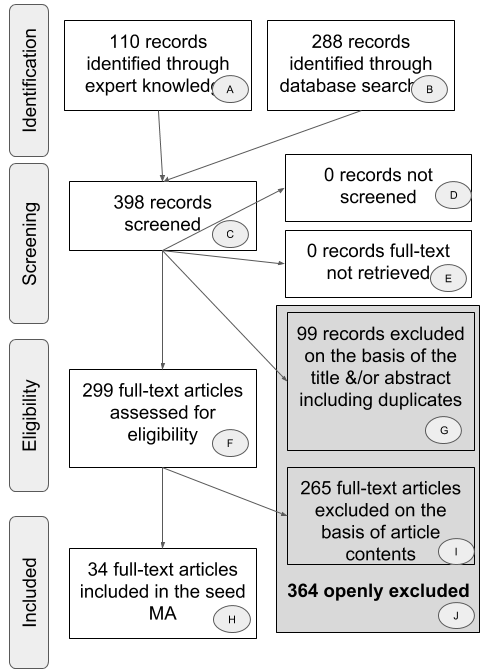
\includegraphics{figures/PRISMA_MA_Mispronunciation.png}
\caption{}
\end{figure}

\subsection{Study Selection}\label{study-selection}

\begin{lltable}


\begin{longtable}{lllll}\noalign{\getlongtablewidth\global\LTcapwidth=\longtablewidth}
\caption{\label{tab:SummaryTable}Summary of all studies.}\\
\toprule
Paper & Publication format & Age & Vocabulary & N Effect Sizes\\
\midrule
Altvater-Mackensen (2010) & dissertation & 22, 25 & None & 13\\
Altvater-Mackensen et al. (2014) & paper & 18, 25 & None & 16\\
Bailey \& Plunkett (2002) & paper & 18, 24 & Comp & 12\\
Ballem \& Plunkett (2005) & paper & 14 & None & 4\\
Bergelson \& Swingley (2017) & paper & 6, 7, 9, 12 & None & 9\\
Bernier \& White (2017) & proceedings & 21 & None & 4\\
Delle Luche et al. (2015) & paper & 20, 19 & None & 4\\
Durrant et al. (2014) & paper & 19, 20 & None & 4\\
Höhle et al. (2006) & paper & 18 & None & 4\\
Højen et al. (n.d.) & gray paper & 19, 20 & Comp/Prod & 6\\
Mani \& Plunkett (2007) & paper & 15, 18, 24, 14, 20 & Comp/Prod & 14\\
Mani \& Plunkett (2010) & paper & 12 & Comp & 8\\
Mani \& Plunkett (2011) & paper & 23, 17 & None & 15\\
Mani, Coleman, \& Plunkett (2008) & paper & 18 & Comp/Prod & 4\\
Ramon-Casas \& Bosch (2010) & paper & 24, 25 & None & 4\\
Ramon-Casas et al. (2009) & paper & 21, 20, 43, 44 & Prod & 14\\
Ren \& Morgan (in press) & gray paper & 19 & None & 8\\
Renner (2017) & dissertation & 17, 24 & None & 6\\
Skoruppa et al. (2013) & paper & 23 & None & 5\\
Swingley (2003) & paper & 19 & Comp/Prod & 6\\
Swingley (2009) & paper & 17 & Comp/Prod & 4\\
Swingley (2016) & paper & 27, 28 & Prod & 9\\
Swingley \& Aslin (2000) & paper & 20 & Comp & 2\\
Swingley \& Aslin (2002) & paper & 15 & Comp/Prod & 4\\
Tamasi (2016) & dissertation & 30 & None & 4\\
Tao \& Qinmei (2013) & paper & 12 & None & 4\\
Tao et al. (2012) & paper & 16 & Comp & 6\\
van der Feest \& Fikkert, (2015) & paper & 24, 20 & None & 16\\
van der Feest \& Johnson (2016) & paper & 24 & None & 24\\
Wewalaarachchi et al. (2017) & paper & 24 & None & 8\\
White \& Aslin (2011) & paper & 18 & None & 4\\
White \& Morgan (2008) & paper & 18, 19 & None & 12\\
Zesiger \& Jöhr (2011) & paper & 14 & None & 8\\
Zesiger et al. (2012) & paper & 12, 19 & Comp/Prod & 6\\
\bottomrule
\end{longtable}
\end{lltable}

We first generated a list of potentially relevant items to be included
in our meta-analysis by creating an expert list. This process yielded
110 items. We then used the google scholar search engine to search for
papers citing the original Swingley \& Aslin (2000) publication. This
search was conducted on 22 September, 2017 and yielded 288 results. We
removed 99 duplicate items and screened the remaining 299 items for
their title and abstract to determine whether each met the following
inclusion criteria: (1) original data was reported; (2) the experiment
examined familiar word recognition and mispronunciations; (3) infants
studied were under 31-months-of-age and typically developing; (4) the
dependent variable was derived from proportion of looks to a target
image versus a distractor in a eye movement experiment; (5) the stimuli
were auditory speech. The final sample (n = \emph{34}) consisted of 28
journal articles, 1 proceedings paper, 3 thesis, and 2 unpublished
reports. We will refer to these items collectively as papers. Table 1
provides an overview of all papers included in the present
meta-analysis.

\subsection{(Insert Table 1 about
here)}\label{insert-table-1-about-here}

\subsection{Data Entry}\label{data-entry}

The 34 papers we identified as relevant were then coded with as much
consistently reported detail as possible (Tsuji, Bergmann, \& Cristia,
2014; Bergmann et al., 2018). For each experiment (note that a paper
typically has multiple experiments), we entered variables describing the
publication, population, experiment design and stimuli, and results. For
the planned analyses to evaluate the development of mispronunciation
sensitivity, we focus on the following characteristics:

1 Condition: Were words mispronounced or not;\\
2 Mean age reported per group of infants, in days;\\
3 Vocabulary size, measured by a standardized questionnaire or list;

We separated conditions according to whether or not the target word was
mispronounced to be able to investigate infants' looking to the target
picture as well as their mispronunciation sensitivity, which is the
difference between looks to the target in correct and mispronounced
trials. When the same infants were further exposed to multiple
mispronunciation conditions and the results were reported separately in
the paper, we also entered each condition as a separate row (e.g.,
consonant versus vowel mispronunciations; Mani \& Plunkett, 2007). The
fact that the same infants contributed data to multiple rows (minimally
those containing information on correct and mispronounced trials) leads
to shared variance across effect sizes, which we account for in our
analyses (see next section). We will call each row a record; in total
there were 271 records in our data.

\subsection{Data analysis}\label{data-analysis}

{[}Christina: I needed to move this around because we first need to say
that we could not compute some effect sizes and removed outlierts.{]}

Effect sizes are reported for infants' looks to target pictures after
hearing a correctly pronounced or a mispronounced label (object
identification) as well as the difference between effect sizes for
correct and mispronounced trials (i.e.~mispronunciation sensitivity).
The effect size reported in the present paper is based on comparison of
means, standardized by their variance. The most well-known effect size
from this group is Cohen's \emph{d} {[}@cohen{]}. To correct for the
small sample sizes common in infant research, however, we used as a
dependent variable Hedges' \emph{g} instead of Cohen's \emph{d} (Hedges,
1981; Morris, 2000).

{[}Katie{]} Do you want number of records and papers for the imputed
correlations as well? You've put a -1, assuming there was something
wrong with one of the papers or something like that? How does that shake
out for number of records? {[}Christina: No clue what the -1 was,
sorry.{]}

We calculated Hedges' \emph{g} using the raw means and standard
deviations reported in the paper (\emph{n} = 186 records from 26 papers)
or using reported t-values (\emph{n} = 74 records from 9 papers). Two
papers reported raw means and standard deviations for some experimental
conditions and just t-values for the remaining experimental conditions
(Swingley, 2016; Altvater-Mackensen et al., 2014). Raw means and
standard deviations were extracted from figures for 4 papers. In a
within-participation design, when two means are compared (i.e.~looking
during pre- and post-naming) it is necessary to obtain correlations
between the two measurements at the participant level to calculate
effect sizes and effect size variance based on t-values. Upon request we
were provided with correlation values for one paper (Altvater-Mackensen,
2010); we were able to compute correlations using means, standard
deviations, and t-values for \emph{n} = 5 (following Csibra, et al.
2016, Appendix B; see also Rabagliati, Ferguson, \& Lew-Williams, 2018).
Correlations were imputed for the remaining papers (see Black \&
Bergmann, 2017, for the same procedure). For two papers, we could not
derive any effect size (Ballem \& Plunkett, Renner), and for a third
paper, we do not have sufficient information in one record to compute
effect sizes (Skoruppa). We compute a total of 106 effect sizes for
correct pronunciations and 150 for mispronunciations. Following standard
meta-analytic practice, we remove outliers, i.e.~effect sizes more than
3 standard deviations from the respective mean effect size. This leads
to the exclusion of 2 records for correct pronunciations and 3 records
for mispronunciations.

To take into account the fact that the same infants contributed to
multiple datapoints, we analyze our results in a multilevel approach
using the R {[}@R{]} package metafor {[}@metafor{]}. This means we model
as random effect that effect sizes from the same paper share are based
on more similar studies than those across papers and that nested therein
effects can stem from the same infants.

{[}Christina: In the above 2 paragraphs I got confused, should it be
present or past. I think it switched in the las tparagraph so I started
to adapt, but I think it would be best for you to decide. {]}{[}Katie:
Good catch. I've gone through the Methods section and changed everything
to past, per APA guidelines.{]}

Mispronunciation sensitivity studies typically examine infants'
proportion of target looks (PTL) in comparison to some baseline
measurement. PTL is calculated by dividing the percentage of looks to
the target by the total percentage of looks to both the target and
distractor images. Across papers the baseline comparison varied; we used
the baseline reported by the authors of each paper. Most papers
(\emph{n} = 52 records from 13 papers) subtracted the PTL score for a
pre-naming phase from the PTL score for a post-naming phase and report a
difference score.

Other papers either compared post- and pre-naming PTL with one another
(\emph{n} = 29 records from 10 papers), thus reporting two variables, or
compared post-naming PTL with a chance level of 50\%, (\emph{n} = 23
records from 9 papers). For all these comparisons, positive values
(either as reported or after subtraction of chance level or a pre-naming
PTL) indicate target looks towards the target object after hearing the
label, i.e.~a recognition effect. Standardized effect sizes based on
mean differences, as calculated here, preserve the sign. Consequently,
positive effect sizes reflect more looks to the target picture after
naming, and larger positive effect sizes indicate comparatively more
looks to the target.

\subsection{Publication Bias}\label{publication-bias}

In the psychological sciences, there is a documented reluctance to
publish null results. As a result, significant results tend to be
over-reported and thus might be over-represented in our meta-analyses
(see Ferguson \& Heene, 2012). To examine whether this is also the case
in the mispronunciation sensitivity literature, which would bias the
data analyzed in this meta-analysis, we conducted two tests. We first
examined whether effect sizes are distributed as expected based on
sampling error using the rank correlation test of funnel plot asymmetry
with the R {[}@R{]} package metafor {[}@metafor{]}. Effect sizes with
low variance were expected to fall closer to the estimated mean, while
effect sizes with high variance should show an increased,
evenly-distributed spread around the estimated mean. Publication bias
would lead to an uneven spread.

Second, we analyze all of the significant results in the dataset using a
p-curve from the p-curve app (v4.0, p-curve.com; @pcurve). This p-curve
tests for evidential value by examining whether the p-values follow the
expected distribution of a right skew in case the alternative hypothesis
is true, versus a flat distribution that speaks for no effect being
present in the population and all observed significant effects being
spurious. Responses to correctly pronounced and mispronounced labels
were predicted to show different patterns of looking behavior. In other
words, there is an expectation that infants should look to the target
when hearing a correct pronunciation, but studies vary in their report
of significant looks to the target when hearing a mispronounced label
(i.e.~there might be no effect present in the population, see e.g., );
as a result, we conducted these two analyses to assess publication bias
separately for both conditions.

\subsection{Meta-analysis}\label{meta-analysis}

The models reported here are hierarchical random-effects models (infant
groups nested within papers) of variance-weighted effect sizes, which we
computed with the R {[}@R{]} package metafor {[}@metafor{]}. To
investigate how development impacts mispronunciation sensitivity, our
core theoretical question, we introduced age (centered; continuous and
measured in days but transformed into months for ease of interpreting
estimates by dividing by 30.44) as a moderator to our main model. For a
subsequent exploratory investigations of experimental characteristics,
we introduced each characteristic as a moderator (more detail below).

\section{Results}\label{results}

\subsection{Publication Bias}\label{publication-bias-1}

Figure 2 shows the funnel plots for both correct pronunciations and
mispronunciations (code adapted from Sakaluk, 2016). Funnel plot
assymmetry was significant for both correct pronunciations (Kendall's
\(\tau\) = 0.53, \emph{p} \textless{} .001) and mispronunciations
(Kendall's \(\tau\) = 0.16, \emph{p} = 0.004). These results,
quantifying the assymmetry in the funnel plots (Figure 1), indicate bias
in the literature. This is particularly evident for correct
pronunciations, where larger effect sizes have greater variance (bottom
right corner) and there are a smaller number of more precise effect
sizes (i.e.~smaller variance) than expected (top left, outside the
triangle).

The stronger publication bias for correct pronunciation might reflect
the status of this condiction as a control. If infants were not looking
to the target picture after hearing the correct label, the overall
experiment design is called into questions. However, due to the small
effect and sample sizes (which we will discuss in the following sections
in more detail) one would expect the regular occurrence of null results
even though as a population infants would reliably show the expected
object identification effect.

We should also point out that funnel plot asymmetry can be caused by
multiple factors beside publication bias, such as heterogeneity in the
data. There are various possible sources of heterogeneity, which our
subsequent moderator analyses will begin to address. Nonetheless, we
will remain cautious in our interpretation of our findings and hope that
an open dataset which can be expanded by the community will attract
previously unpublished null results so we can better understand infants'
developing mispronunciation sensitivity.

\subsection{(Insert Figure 2 about
here)}\label{insert-figure-2-about-here-1}

\begin{verbatim}
## pdf 
##   2
\end{verbatim}

\begin{figure}
\centering
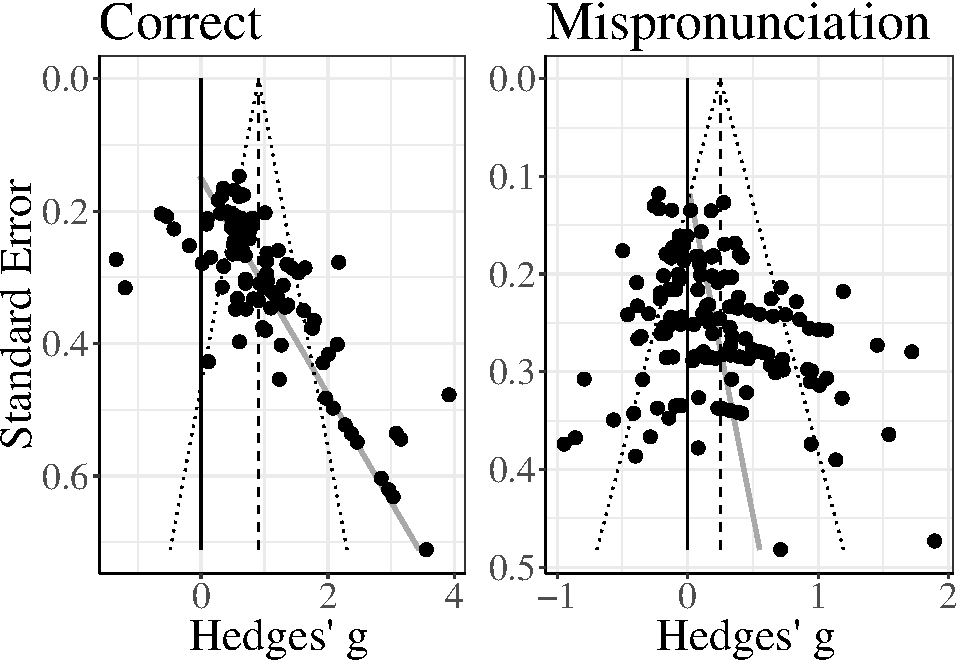
\includegraphics{Paper_Analyses_files/figure-latex/FunnelCombo-1.pdf}
\caption{}
\end{figure}

\begin{verbatim}
## [1] TRUE
\end{verbatim}

\begin{verbatim}
## [1] TRUE
\end{verbatim}

We next examined the p-curves for significant values from the correctly
pronounced and mispronounced conditions. The p-curve based on 72
statistically significant values for correct pronunciations indicates
that the data contain evidential value (Z = -17.93, \emph{p} \textless{}
.001) and we find no evidence of a large proportion of p-values just
below the typical alpha threshold of .05 that researchers consistently
apply in this line of research. The p-curve based on 36 statistically
significant values for mispronunciations indicates that the data contain
evidential value (Z = -6.81, \emph{p} \textless{} .001) and there is
again no evidence of a large proportion of p-values just below the
typical alpha threshold of .05.

Taken together, the results suggest a tendency in the literature towards
publication bias. As a result, our meta-analysis may systematically
overestimate effect sizes and we therefore interpret all estimates with
caution. Yet, the p-curve analysis suggests that the literature contains
evidential value, reflecting a \enquote{real} effect. We therefore
continue our meta-analysis.

\subsection{Meta-analysis}\label{meta-analysis-1}

\subsubsection{Object Identification for Correct and Mispronounced
Words}\label{object-identification-for-correct-and-mispronounced-words}

We first calculated the meta-analytic effect for infants' ability to
identify objects when hearing correctly pronounced labels. The
variance-weighted meta-analytic effect size Hedges' \emph{g} was 0.908
(SE = 0.12) which was significantly different from zero (CI {[}0.673,
1.143{]}, \emph{p} \textless{} .001). This is a rather large effect size
(according to the criteria set by Cohen, 1988; see also Bergmann, et
al., 2018; for comparative meta-analytic effect sizes in language
acquisition research). That the effect size is significantly above zero
suggests that when presented with the correctly pronounced label,
infants fixated the corresponding object. Our analysis of funnel plot
asymmetry, however, found evidence for publication bias, which might
lead to an overestimated effect sizes as smaller, non-significant
results might not be published despite the fact that they should occur
regularly even in well-powered studies. Although the effect size Hedges'
\emph{g} may be overestimated for object identification in response to
correctly pronounced words, the p-curve results and a CI lower bound of
0.67, which is substantially above zero, together suggest that this
result is somewhat robust. In other words, we are confident that the
true population mean lies above zero for object recognition of correctly
pronounced words.

We then calculated the meta-analytic effect for object identification in
response to mispronounced words. In this case, the variance-weighted
meta-analytic effect size Hedges' \emph{g} was 0.25 (SE = 0.06) which
was also significantly different from zero (CI {[}0.133, 0.367{]},
\emph{p} \textless{} .001). This is considered a small effect size
(Cohen, 1988), but significantly above zero, which suggests that even
when presented with a mispronounced label, infants fixated the correct
object. In other words, infants are able to resolve mispronunciations, a
key skill in language processing We again note the publication bias
(which was smaller in this condition), and the possibility that the
effect size Hedges' \emph{g} may be overestimated. But, as the p-curve
indicated evidential value, we are confident in the overall patterns,
namely that infants fixate the target even after hearing a mispronounced
label.

\subsubsection{Mispronunciation Sensitivity Meta-analytic
Effect}\label{mispronunciation-sensitivity-meta-analytic-effect}

The above two analyses considered the data from mispronounced and
correctly pronounced words separately. To evaluate mispronunciation
sensitivity, we compared the effect size Hedges' \emph{g} for correct
pronunciations with mispronunciations directly. To this end, we combined
the two datasets. The moderator test was significant, QM(1) = 215.761,
\emph{p} \textless{} .001. The estimate for mispronunciation sensitivity
was 0.495 (SE = 0.034), and infants' looking times across conditions
were significantly different (CI {[}0.429, 0.561{]}, \emph{p}
\textless{} .001). This confirms that although infants fixate the
correct object for both correct pronunciations and mispronunciations,
the observed fixations to target (as measured by the effect sizes) were
significantly greater for correct pronunciations. In other words, we
observe a significant difference between the two conditions and can now
quantify the modulation of fixation behavior in terms of standardized
effect sizes and their variance. This first result has both theoretical
and practical implications, as we can now reason about the amount of
perturbance caused by mispronunciations and can plan future studies to
further investigate this effect with suitable power.

Heterogeneity was significant for both correctly pronounced (Q(103) =
625.63, \emph{p} \textless{} .001) and mispronounced words, (Q(146) =
462.51, \emph{p} \textless{} .001), as well as mispronunciation
sensitivity, which included the moderator condition, (QE(249) =
1,088.14, \emph{p} \textless{} .001). This indicated that the sample
contains unexplained variance leading to significant difference across
our studies beyond what is to be expected based on random sampling
error. We therefore continue with our moderator analysis to investigate
possible sources of this variance.

\subsubsection{Object Recognition and Mispronunciation Sensitivity
Modulated by
Age}\label{object-recognition-and-mispronunciation-sensitivity-modulated-by-age}

To evaluate the different predictions we laid out in the introduction
for how mispronunciation sensitivity will change as infants develop, we
next added the moderator age (centered; continuous and measured in days
but transformed into months for ease of interpreting estimates by
dividing by 30.44 for Figure 3).

In the first analyses, we investigate the impact of age separately on
conditions where words were either pronounced correctly or not. Age did
not significantly modulate object identification in response to
correctly pronounced (QM(1) = 0.678, \emph{p} = 0.41) or mispronounced
words (QM(1) = 1.715, \emph{p} = 0.19). The lack of a significant
modulation together with the small estimates (correct: \(\beta\) =
0.015, SE = 0.018, 95\% CI{[}-0.02, 0.049{]}, \emph{p} = 0.41;
mispronunciation: \(\beta\) = 0.015, SE = 0.011, 95\% CI{[}-0.007,
0.037{]}, \emph{p} = 0.19) indicates that there was no relationship
between age and target looks in response to a correctly pronounced or
mispronounced label. We plot both object recognition and
mispronunciation sensitivity as a function of age in Figure 3.

We then examined the interaction between age and mispronunciation
sensitivity (correct vs.~mispronounced words) in our whole dataset. The
moderator test was significant (QM(3) = 218.621, \emph{p} \textless{}
.001). The interaction between age and mispronunciation sensitivity,
however, was not significant (\(\beta\) = 0.003, SE = 0.008, 95\%
CI{[}-0.012, 0.018{]}, \emph{p} = 0.731); the moderator test was mainly
driven by the difference between conditions. The small estimate, as well
as inspection of Figure 2 suggests that as infants age, their
mispronunciation sensitivity remains the same.

\subsection{(Insert Figure 3 about
here)}\label{insert-figure-3-about-here}

{[}Christina{]} Can you try and align the axes for both plots?
{[}Katie{]} I can, but then the dotted line doesn't extend the full way
(which I think is quite ugly). Not sure how to fix that.

\begin{verbatim}
## pdf 
##   2
\end{verbatim}

\begin{figure}
\centering
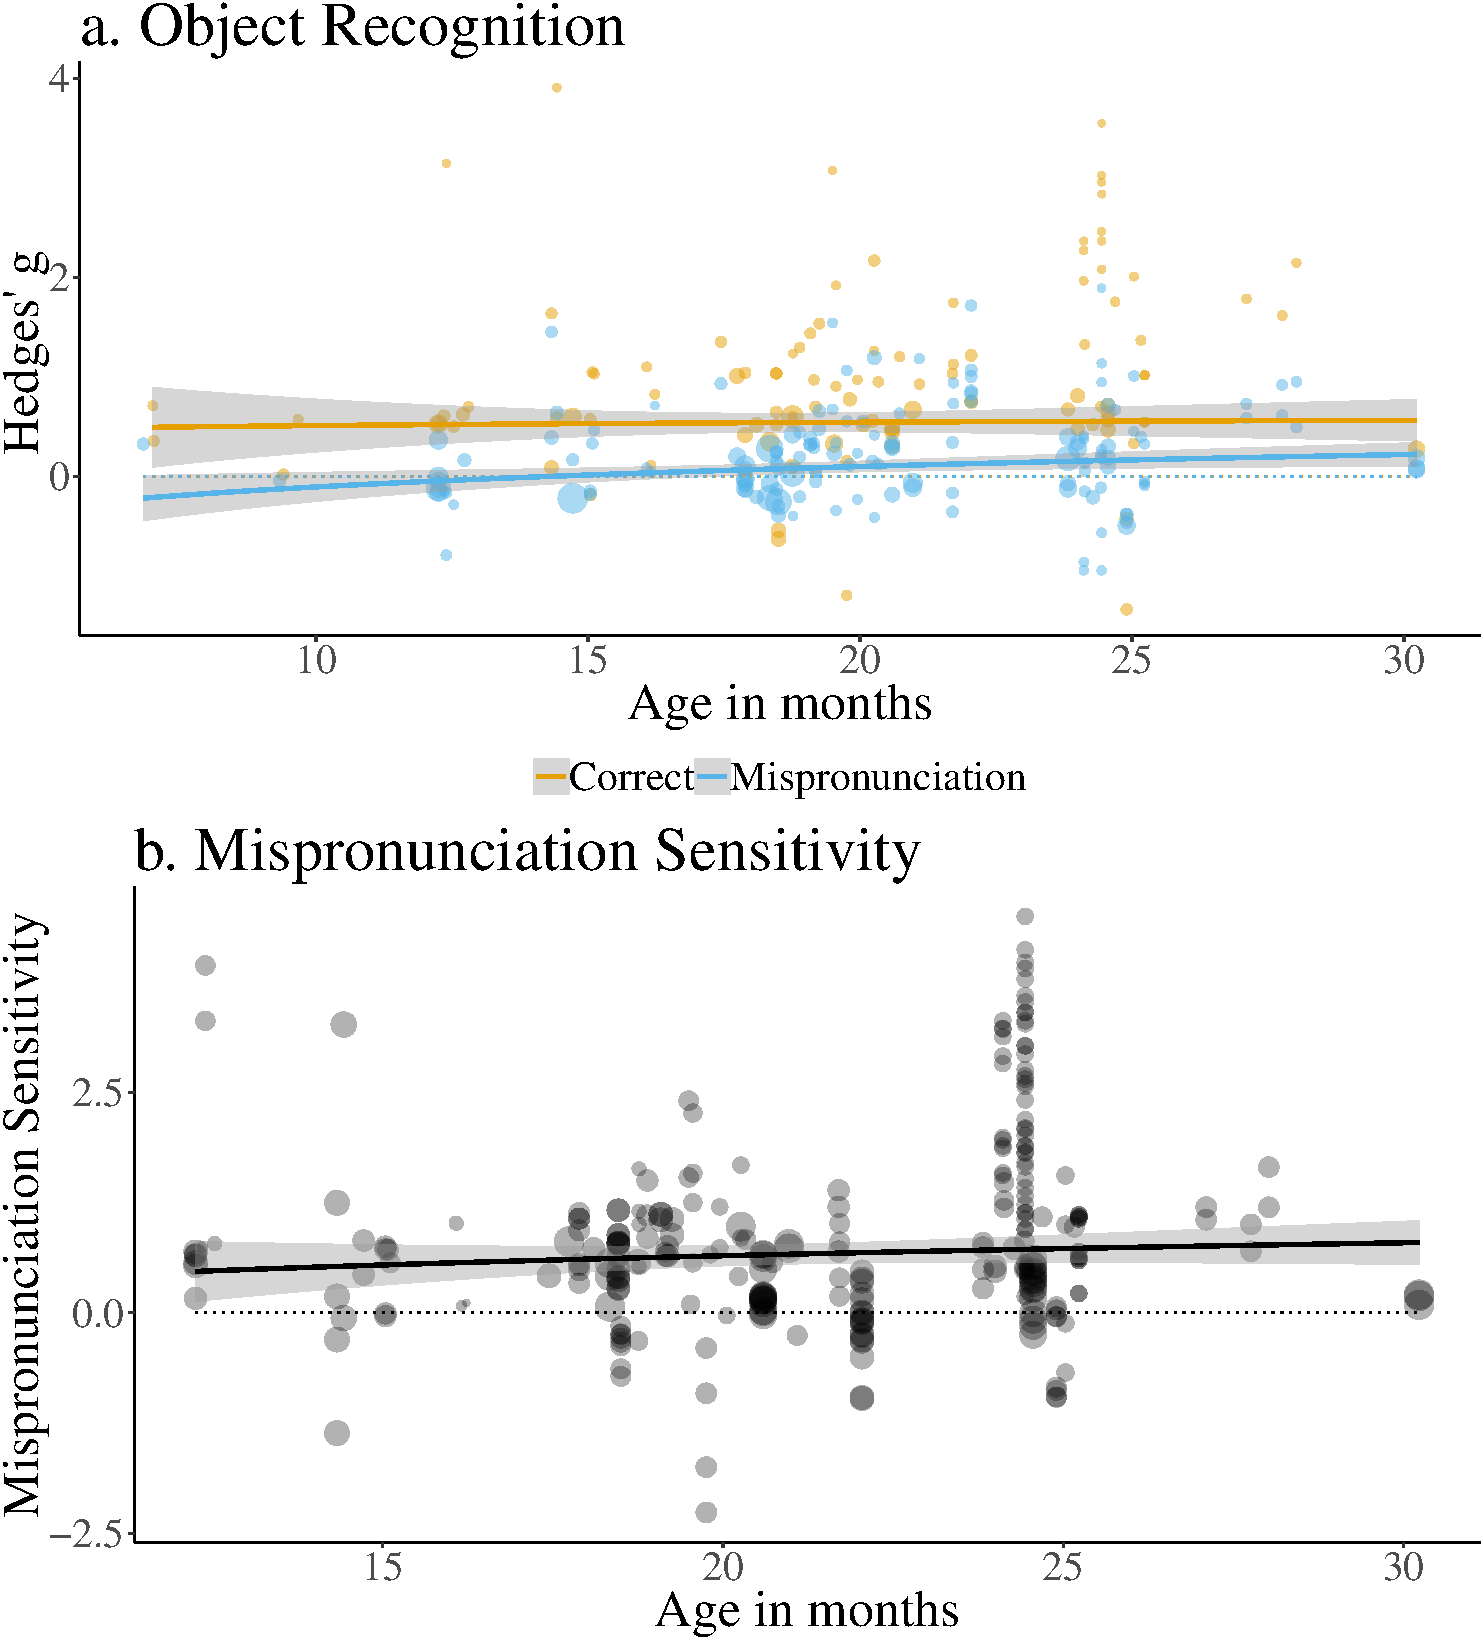
\includegraphics{Paper_Analyses_files/figure-latex/PlotMPEffect-1.pdf}
\caption{}
\end{figure}

\subsubsection{Vocabulary Size: Correlation Between Mispronunciation
Sensitivity and
Vocabulary}\label{vocabulary-size-correlation-between-mispronunciation-sensitivity-and-vocabulary}

Of the 32 papers included in the meta-analysis, 13 analyzed the
relationship between vocabulary scores and object recognition for
correct pronunciations and mispronunciations (comprehension = 11 papers
and 39 records; production = 3 papers and 20 records). There is reason
to believe that production data are different from comprehension data
(the former being easier to estimate for parents in the typical
questionnaire-based assessment; Tomasello \& Mervis, 1994), and we
therefore planned to analyze these two types of vocabulary measurement
separately. However, because only 3 papers reported correlations with
productive vocabulary scores, only limited conclusions that can be
drawn. In our vocabulary analysis, we therefore focus exclusively on the
relationship between comprehension and mispronunciation sensitivity.

{[}Katie: Tomasello reference -
\url{https://onlinelibrary.wiley.com/doi/abs/10.1111/j.1540-5834.1994.tb00186.x}{]}

We first considered the relationship between vocabulary and object
recognition for correct pronunciations. Higher comprehension scores were
associated with greater object recognition in response to correct
pronunciations for 9 of 10 experimental conditions, with correlation
values ranging from -0.16 to 0.48. The mean effect size Pearson's
\emph{r} of 0.14 was small but did differ significantly from zero (CI
{[}0.03; 0.25{]} \emph{p} = 0.012). However, the lower bound of the CI
is close to zero and considering the small sample size, one might
hypothesize that with more power the small relationship might become
even larger. As a result, we can draw a tentative conclusion that there
is a positive relationship between comprehension scores and object
recognition in response to correct pronunciations.

{[}Christina{]} It's significant now! {[}Katie{]} Must be because you
removed the outliers. I've changed around the wording :)

We next considered the relationship between vocabulary and object
recognition for mispronunciations. Higher comprehension scores were
associated with greater object recognition in response to correct
pronunciations for 17 of 29 experimental conditions, with correlation
values ranging from -0.35 to 0.57. The mean effect size Pearson's
\emph{r} of 0.05 was small and did not differ significantly from zero
(CI {[}-0.01; 0.12{]} \emph{p} = 0.119). The small correlation and large
variances suggest a lack of relationship between vocabulary and object
recognition for mispronunciations. We again emphasize that we cannot
draw a firm conclusion due to the small number of studies we were able
to include here.

Figure 4 plots the year of publication for all the mispronunciation
sensitivity studies included in this meta-analysis. This figure
illustrates two things: the growing number of mispronunciation
sensitivity studies and the waning number of studies measuring
vocabulary. The lack of evidence for a relationship between
mispronunciation sensitivity and vocabulary size in early studies may
have contributed to increasingly fewer researchers including vocabulary
measurements in their mispronunciation sensitivity experimental design.
This may explain our underpowered analysis of the relationship between
mispronunciation sensitivity and vocabulary size.

\subsection{(Insert Figure 4 about
here)}\label{insert-figure-4-about-here}

\begin{figure}
\centering
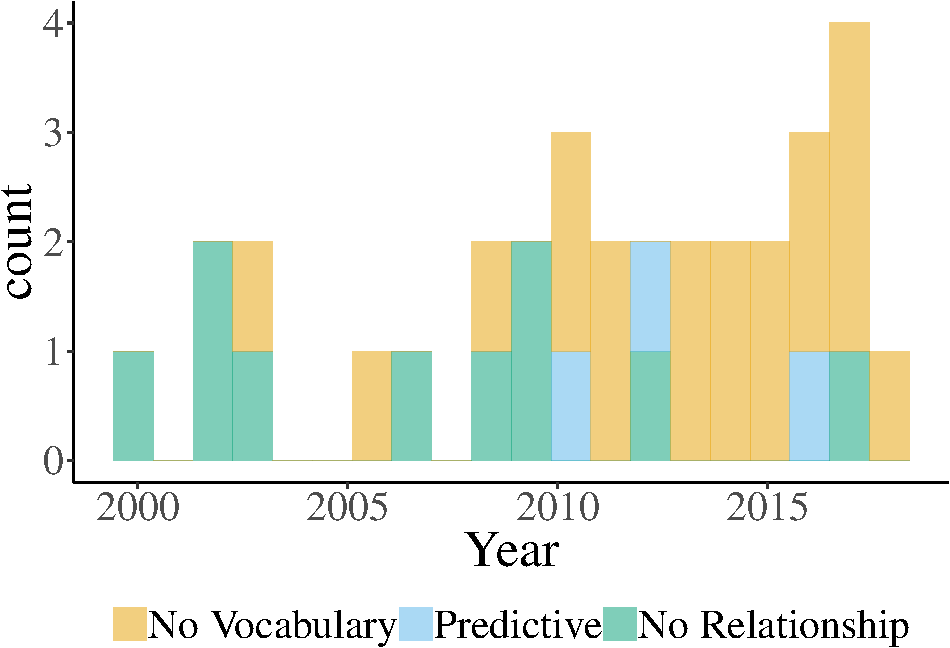
\includegraphics{Paper_Analyses_files/figure-latex/Vocab_describe1-1.pdf}
\caption{}
\end{figure}

\begin{verbatim}
## pdf 
##   2
\end{verbatim}

\subsubsection{Interim Discussion}\label{interim-discussion}

The main goal of this paper was to assess mispronunciation sensitivity
and its maturation with age. The results seem clear: Although infants
consider a mispronunciation as a better match with the target image than
a distractor image, there was a consistent effect of mispronunciation
sensitivity. This did not change with development nor with vocabulary
size. Of the 3 predictions and assumptions about the development of
infants' sensitivity to mispronunciations discussed in the Introduction,
the present results lend some support for the argument that
mispronunciation sensitivity stays consistent as infants develop. This
runs counter to existing theories of phono-lexical development, which
predict either an increase (PRIMR ref) or decrease (Assim Model ref) in
mispronunciation sensitivity. Furthermore, although we found a
relationship between vocabulary comprehension and target looking for
correct pronunciations, we found no relationship between vocabulary and
target looking for mispronunciations. This also runs counter to the
predictions for the PRIMR (PRIMR ref) and Assimilation (Assim ref)
models, but may be due to our analyses being underpowered. In sum, it
seems that current theories of infants' phono-lexical development cannot
fully capture our results, but that more investigation is needed to draw
a firm conclusion.

Alternatively, an effect of maturation might have been masked by other
factors we have not yet captured in our analyses. A strong candidate
that emerged during the construction of the present dataset and careful
reading of the original papers is the analysis approach. We observed, as
mentioned in the Methods section, large variance in the dependent
variable reported, and additionally noted variance in the size of the
time window chosen for analyses. Researchers might adapt their analysis
strategy to age or they might be influenced by having observed the data.
In the latter case, we expect an increase in significant results, which
at the same time can (partially) explain the publication bias we observe
(Simmons, Nelson, \& Simonsohn, 2011).

We included details related to timing and type of dependent variable
calculated in our coding of the dataset because they are consistently
reported and might be useful for experiment design in the future by
highlighting typical choices and helping establish field standards. In
the following section, we include an exploratory analysis to investigate
the possibility of systematic differences in the approach to analysis in
general and across infant age. The purpose of this analysis is to better
understand the influence of choices made in analyzing mispronunciation
sensitivity studies as well as the influence these choices may have on
our understanding of mispronunciation sensitivity development.

\subsection{Exploratory Analyses}\label{exploratory-analyses}

We identified two sets of variables which had the potential to vary
across papers to assess the influence of data analysis choices on
resulting effect size: timing (size of time window analyzed; offset
time) and which dependent variable(s) were reported. In the following,
we discuss the possible theoretical motivation for these data analysis
choices, the variation present in the current meta-analysis dataset, and
the influence these analysis choices have on mispronunciation
sensitivity development. We focus specifically on the size of the
mispronunciation sensitivity effect, considering the whole dataset and
including condition (correct pronunciation, mispronunciation) as
moderator.

\subsubsection{Timing}\label{timing}

In a typical trial in a mispronunciation sensitivity study, the
target-distractor image pairs are first presented in silence, followed
by auditory presentation of a carrier phrase or isolated presentation of
the target word (correctly pronounced or mispronounced). When designing
mispronunciation sensitivity studies, experimenters can choose the
length of time each trial is presented. This includes both the length of
time before the target object is named (pre-naming phase) as well as
after (post-naming phase) and is determined prior to data collection. To
examine the size of the time window analyzed in the post-naming phase,
we must first consider overall length of time post-naming, because it
limits the overall time window available to analyze and might thus
predict which time window was analyzed. Across papers, actual
post-naming phase length varied from 2000 to 9000 ms, with a median
value of 3500 ms. We note that the most popular actual post-naming phase
length was 4000 ms, used in \emph{n} = 74 experimental conditions. There
was an inverse relationship between infant age and actual post-naming
phase length, such that younger infants were presented with longer a
longer post-naming phase, although this correlation was not significant
(\emph{r} = 0.01, \emph{p} = 0.882). Presumably, younger infants may be
exposed to longer trials because their word recognition abilities are
expected to be slower than older infants (Fernald et al., 1998).

Unlike the actual post-naming phase length, the size of the post-naming
time window analyzed can be chosen after the experimental data is
collected. Interestingly, half of the experimental conditions were
analyzed using the same length of post-naming phase as the infant heard
in the actual experiment (124), while the other half were analyzed using
a shorter length of post-naming phase, excluding later portions of the
post-naming phase (127). Across papers, the length of the post-naming
phase analyzed varied from 1510 to 4000 ms, with a median value of 2500
ms. We note that the most popular actual post-naming phase length was
2000 ms, used in \emph{n} = 97 experimental conditions. Similar to
actual post-naming phase length, there was an inverse relationship
between infant age and the size of the post-naming time window analyzed,
such that younger infants' looking times were analyzed using a longer
post-naming time window, here the relationship was significant (\emph{r}
= -0.23, \emph{p} \textless{} .001). Again, the choice to analyze a
shorter post-naming time window is likely related to evidence that speed
of processing is slower in younger infants (Fernald et al., 1998). To
summarize, we observe variation in time-related aspects related to
infants' age. This variation is most pronounced, and even significant,
for the time window that is being analyzed after the target label has
been heard.

Another potential source of variation in studies that analyze
eye-movements is the amount of time it takes for an eye movement to be
initiated in response to a visual stimulus, which we refer to as offset
time. Previous studies examining simple stimulus response latencies
first determined that infants require at least 233 ms to initiate an
eye-movement in response to a stimulus (Canfield \& Haith, 1991). In the
first infant mispronunciation sensitivity study, Swingley and Aslin
(2000) used an offset time of 367 ms, which was \enquote{an
\enquote{educated guess} based on studies\ldots{} showing that target
and distractor fixations tend to diverge at around 400 ms.} (Swingley \&
Aslin, 2000, p.~155). Upon inspecting the offset time values used in the
papers in our meta-analysis, the majority used a similar offset time
value (between 360 and 370 ms) for analysis (\emph{n} = 151), but offset
values ranged from 0 to 500 ms, and were not reported for 36
experimental conditions. We note that Swingley (2009) also included
offset values of 1133 ms to analyze responses to coda mispronunciations.
There was an inverse relationship between infant age and size of offset,
such that younger infants were given longer offsets, although this
correlation was not significant (\emph{r} = -0.10, \emph{p} = 0.13).
This lack of a relationship is possibly driven by the field's consensus
that an offset of about 367 ms is appropriate for analyzing word
recognition with PTL measures, including studies that evaluate
mispronunciation sensitivity.

Although there are a priori reasons to choose the post-naming time
window (infant age) or offset time (previous studies), these choices may
occur after data collection and might therefore lead to a higher rate of
false-positives (Gelman, A., \& Loken, E. (2013). Considering that these
choices were systematically different across infant ages, at least for
the post-naming time window, we next explored whether the size of time
window analyzed or the offset time influenced sensitivity to
mispronunciations.

\paragraph{Size of post-naming time window
analyzed}\label{size-of-post-naming-time-window-analyzed}

We first assessed whether size of the post-naming time window analyzed
had an impact on the overall size of the reported mispronunciation
sensitivity. We considered data from both conditions in a joint analysis
and included condition (correct pronunciation, mispronunciation) as an
additional moderator. The moderator test was significant, QM(3) =
236.958, \emph{p} \textless{} .001. The estimate for the interaction
between post-naming phase size and condition was small but significant
\(\beta\) = -0.262, SE = 0.059, 95\% CI{[}-0.377, -0.148{]}, \emph{p}
\textless{} .001. This relationship is plotted in Figure 3a. The results
suggest that the size of the post-naming phase analyzed significantly
impacted mispronunciation sensitivity. Specifically, the difference
between target fixations for correctly pronounced and mispronounced
items (mispronunciation sensitivity) was significantly greater when the
post-naming phase that was shorter in length.

Considering that we also found a relationship between the length of the
post-naming time window analyzed and infant age, such that younger ages
had a longer window of analysis, we next examined whether the size of
post-naming time window analyzed modulated the development of
mispronunciation sensitivity. We merged the two datasets and included
condition (correct pronunciation, mispronunciation) as well as age as
additional moderators. The moderator test was significant QM(7) =
247.322, \emph{p} \textless{} .001. The estimate for the
three-way-interaction between condition, size of post-naming phase, and
age was small, but significant (\(\beta\) = = -0.04, SE = 0.014, 95\%
CI{[}-0.068, -0.012{]}, \emph{p} = 0.006. As can be seen in Figure 3b,
smaller post-naming time window size leads to greater increases in
mispronunciation sensitivity with development. For example, when
experimental conditions were analyzed with a post-naming time window of
2000 ms or less, mispronunciation sensitivity is found to increase with
infant age. If the post-naming time window analyzed is greater than 2000
ms, however, there is no or a negative relation of mispronunciation
sensitivity and age. In other words, all three possible hypotheses might
be supported depending on analysis choices made regarding the size of
the post-naming time window to analyze. This is especially important,
considering that our key question is how mispronunciation sensitivity
changes with development. These results suggest that conclusions about
the relationship between infant age and mispronunciation sensitivity may
be mediated by the size of the post-naming time window analyzed.

\subsection{(Insert Figure 5 about
here)}\label{insert-figure-5-about-here}

\begin{verbatim}
## pdf 
##   2
\end{verbatim}

\begin{figure}
\centering
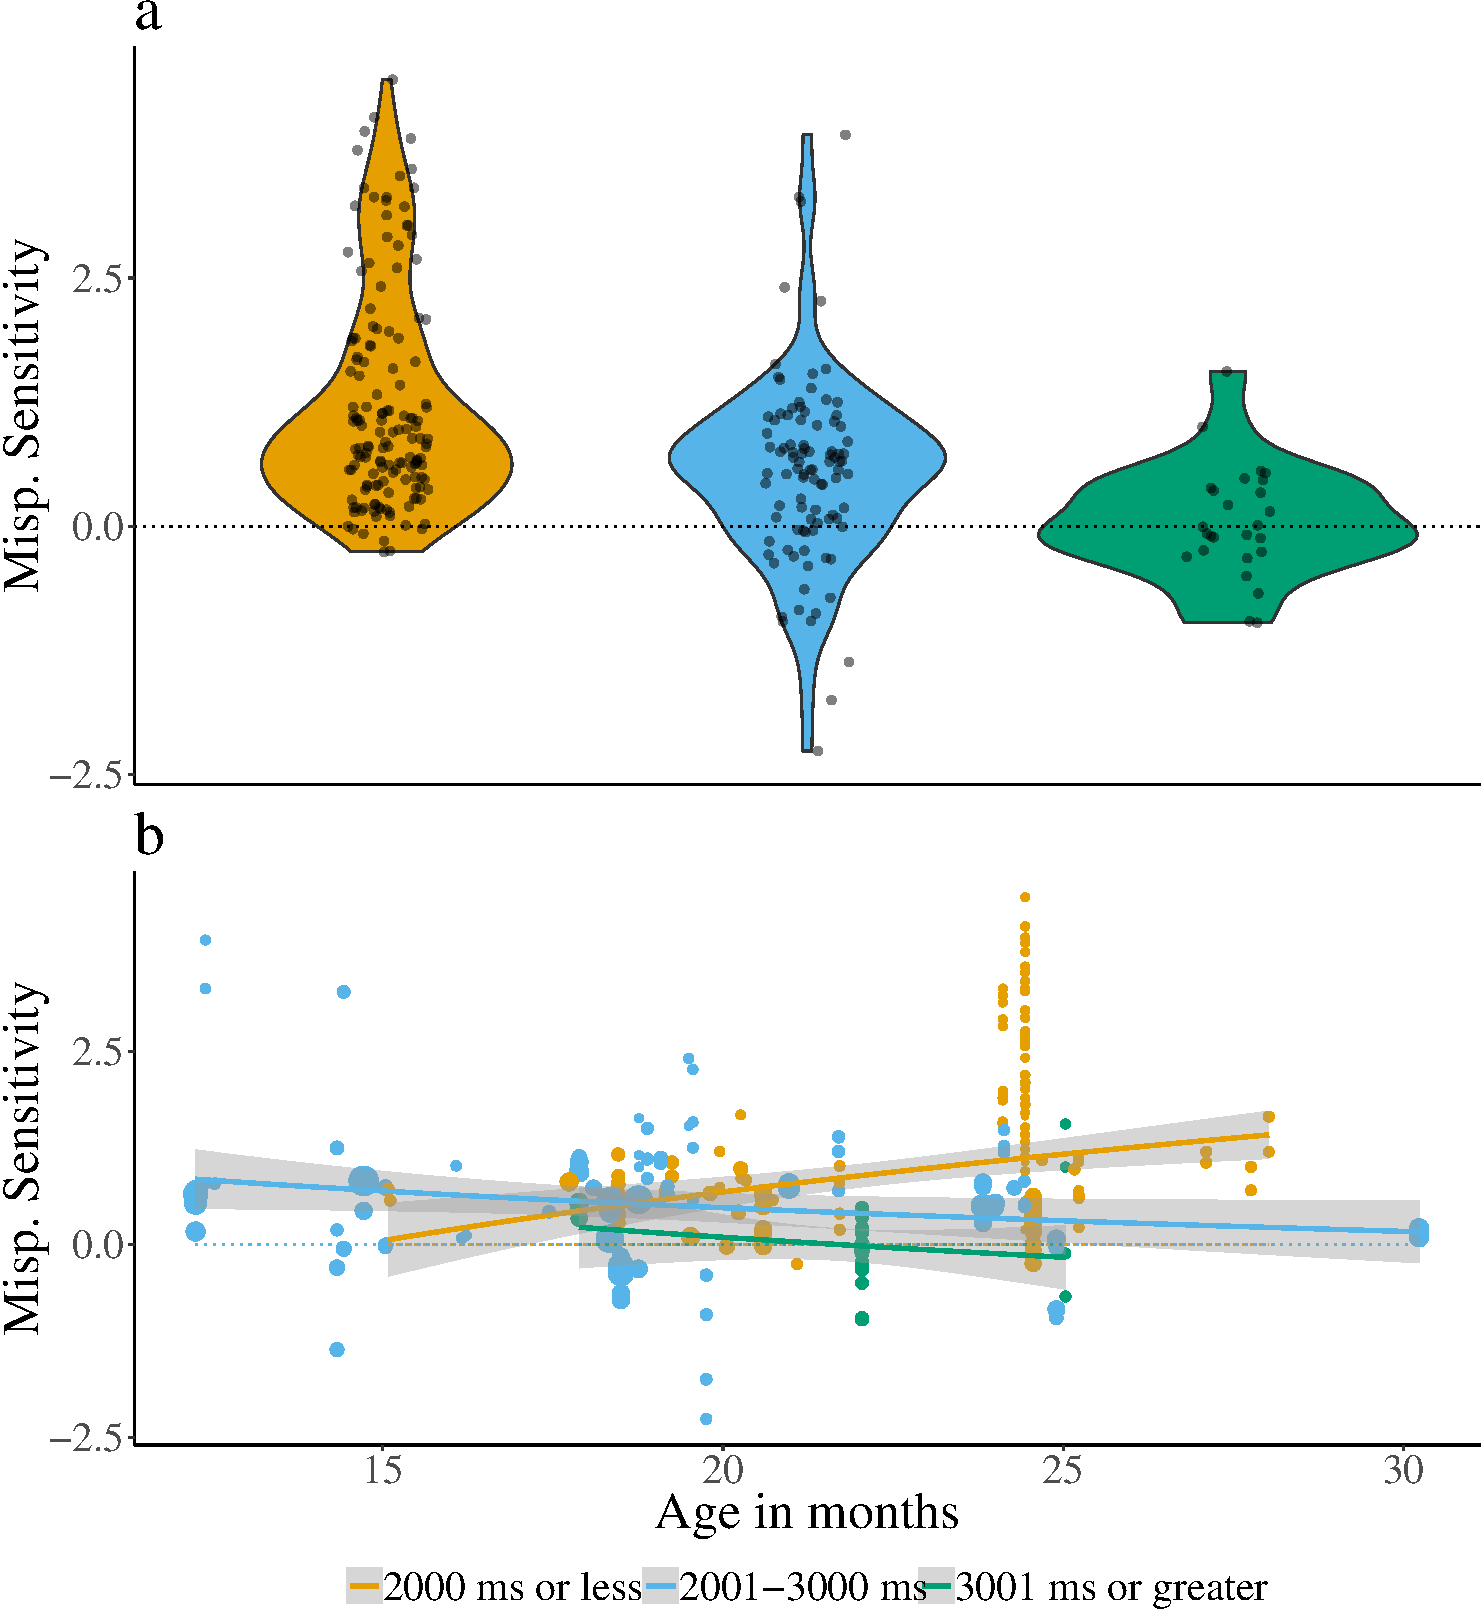
\includegraphics{Paper_Analyses_files/figure-latex/Plot_post_name_cond_age-1.pdf}
\caption{}
\end{figure}

\paragraph{Offset time after target
naming}\label{offset-time-after-target-naming}

We next assessed whether the time between the target was named and the
start of the analysis, namely offset time, had an impact on the size of
the reported mispronunciation sensitivity. When we included both
condition and offset time as moderators, the moderator test was
significant, QM(3) = 236.958, \emph{p} \textless{} .001, but the
estimate for the interaction between offset time and condition was
almost zero \(\beta\) = 0, SE = 0, 95\% CI{[}-0.001, 0{]}, \emph{p} =
0.505. Although we found no relationship between offset time and infant
age, we also examined whether the size of offset time modulated the
development of mispronunciation sensitivity. When both offset time and
condition were included as moderators, the moderator test was
significant QM(7) = 200.867, \emph{p} \textless{} .001, but the
three-way-interaction between condition, offset time, and age was very
small and not significant (\(\beta\) = = 0, SE = 0, 95\% CI{[}0, 0{]},
\emph{p} = 0.605. Taken together, these results suggest that offset time
does not modulate mispronunciation sensitivity. There is no relationship
between offset time and age, and we find no influence of offset time on
the development of mispronunciation sensitivity.

\subsubsection{Dependent variable-related
analyses}\label{dependent-variable-related-analyses}

Mispronunciation studies evaluate infants' proportion of target looks
(PTL) in response to correct and mispronounced words. Experiments
typically include a phase where no naming event has occured, whether
correctly pronounced or mispronounced, which we refer to as the
baseline. The purpose of the baseline is to ensure that infants do not
have systematic preferences for the target or distractor (greater
interest in a cat compared to a cup) which may drive PTL scores in the
post-naming phase. As described in the Data Analysis sub-section of the
Methods, there was considerable variation across papers in way that
baseline was calculated, resulting in different measured outcomes or
dependent variables. Over half of the experimental conditions (\emph{n}
= 129) subtracted the PTL score for a pre-naming phase from the PTL
score for a post-naming phase. This results in one value, which is then
compared with a chance value of 0. When positive, this indicates that
infants increased their looks to the target after hearing the naming
label (correct or mispronounced) relative to the pre-naming baseline
PTL. We will refer to this dependent variable as the Difference Score.
Another dependent variable, which was used in 69 experimental
conditions, directly compared the post- and pre-naming PTL scores with
one another. This requires two values, one for the pre-naming phase and
one for the post-naming phase. A greater post compared to pre-naming
phase PTL indicates that infants increased their target looks after
hearing the naming label. We will refer to this dependent variable as
Pre vs.~Post. Finally, the remaining 53 experimental conditions compared
the post-naming PTL score with a chance value of 50\%. Here, the
infants' pre-naming phase preferences are not considered and instead
target fixations are evaluated based on the likelihood to fixate one of
two pictures. We will refer to this dependent variable as Post.

The Difference Score and Pre vs.~Post can be considered similar to one
another, in that they are calculated on the same type of data and
consider pre-naming preferences. The Post dependent variable, in
contrast, does not consider pre-naming preferences. To our knowledge,
there is no theory or evidence that explicitly drives choice of
dependent variable in analysis of mispronunciation sensitivity, which
may explain the wide variation in dependent variable reported in the
papers included in this meta-analysis. We next explored whether the type
of dependent variable calculated influenced sensitivity to
mispronunciations. Considering that the dependent variable Post differs
in its consideration of pre-naming preferences, we directly compared
mispronunciation sensitivity between Post as a reference condition and
both Difference Score and Pre vs.~Post dependent variables.

We first assessed whether the choice of dependent variable had an impact
on the size of mispronunciation sensitivity. When we included both
condition and dependent variable as moderators, the moderator test was
significant QM(5) = 259.817, \emph{p} \textless{} .001. The estimate for
the interaction between Pre vs.~Post and condition was significantly
smaller than that of the Post dependent variable (\(\beta\) = -0.392, SE
= 0.101, 95\% CI{[}-0.59, -0.194{]}, \emph{p} \textless{} .001), but the
difference between the Difference Score and Post in the interaction with
condition was small and not significant (\(\beta\) = -0.01, SE = 0.098,
95\% CI{[}-0.203, 0.183{]}, \emph{p} = 0.916). This relationship is
plotted in Figure 4a. The results suggest that dependent variable
calculated significantly impacted the size fo the mispronunciation
sensitivity effect, such that Post. vs.~Pre showed a smaller
mispronunciation sensitivity effect than Post, but no difference between
the Difference Score and Post.

We next examined whether the type of dependent variable calculated
modulated the development of mispronunciation sensitivity. When age was
included as an additional moderator, the moderator test was significant
QM(11) = 273.585, \emph{p} \textless{} .001. The estimate for the
interaction between Pre vs.~Post, condition, and age was significantly
smaller than that of the Post dependent variable (\(\beta\) = -0.089, SE
= 0.03, 95\% CI{[}-0.148, -0.03{]}, \emph{p} = 0.003), but the
difference between the Difference Score and Post in the interaction with
condition and age was small and not significant (\(\beta\) = -0.036, SE
= 0.027, 95\% CI{[}-0.088, 0.016{]}, \emph{p} = 0.174). This
relationship is plotted in Figure 4b. When the dependent variable was
Pre vs.~Post, mispronunciation sensitivity decreased with infant age,
while in comparison, when the dependent variable was Post,
mispronunciation sensitivity increased with infant age. There was no
difference in mispronunciation sensitivity change with infant
development between the Post and Difference Score dependent variables.
Similar to size of post-naming time window analyzed, all three possible
developmental hypotheses might be supported depending on the dependent
variable reported. In other words, choice of dependent variable may
influence the conclusion drawn regarding how mispronunciation
sensitivity may change with infant age.

\subsection{(Insert Figure 6 about
here)}\label{insert-figure-6-about-here}

\begin{verbatim}
## pdf 
##   2
\end{verbatim}

\begin{figure}
\centering
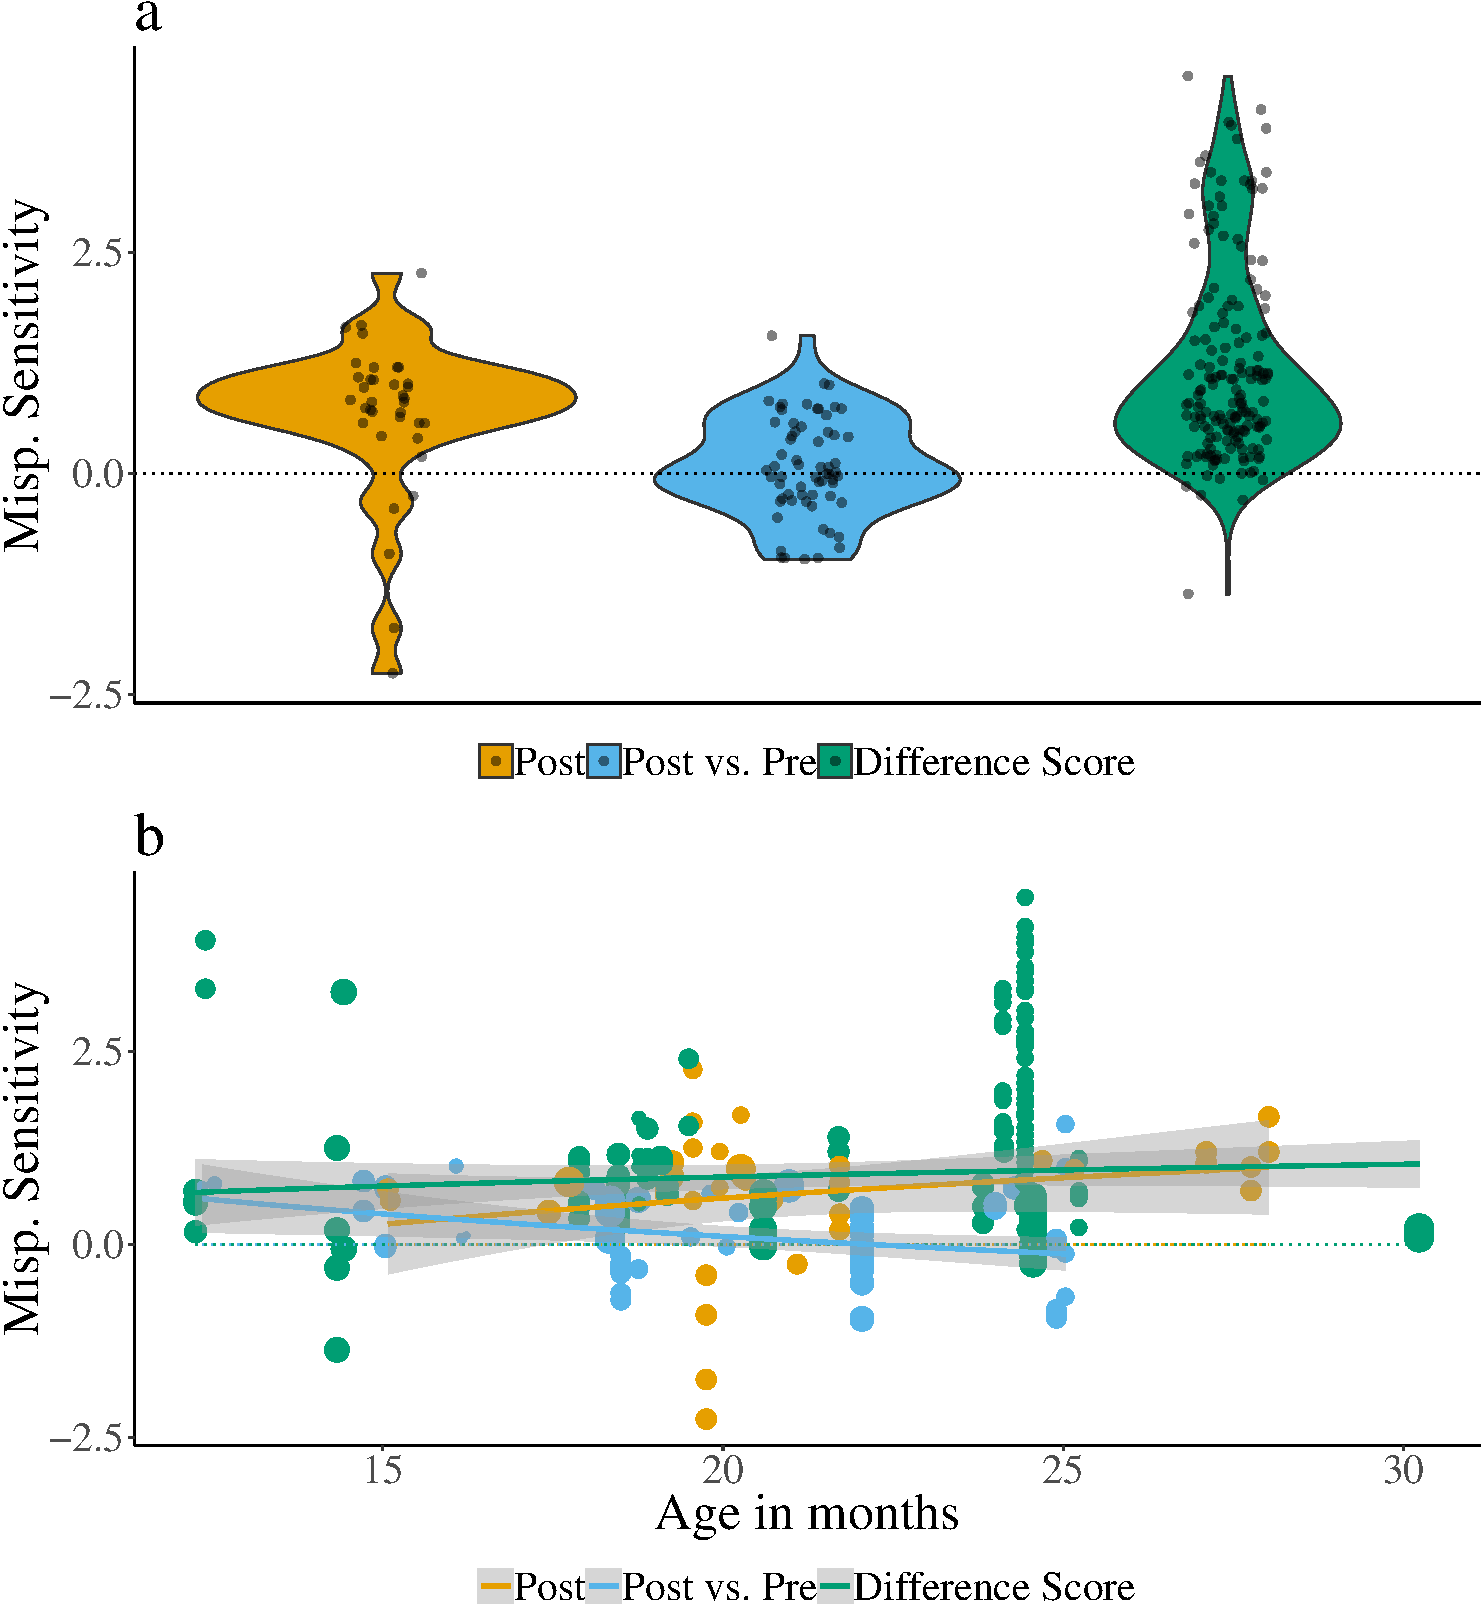
\includegraphics{Paper_Analyses_files/figure-latex/Plot_Within_cond_age_diff_score-1.pdf}
\caption{}
\end{figure}

\section{General Discussion}\label{general-discussion}

Overall, infants showed reliable correct object recognition when given
both correctly pronounced and mispronounced labels. In other words, not
only did infants correctly recognize object labels when they were
correctly pronounced, they also were likely to accept mispronunciations
as acceptable labels for targets. Mispronounced labels were considered a
better match for target images than a distractor image, despite the
differences in the phonological form of correctly pronounced and
mispronounced words. Nonetheless, there was a considerable difference in
target fixations in response to correctly pronounced and mispronounced
labels, suggesting overall mispronunciation sensitivity in the current
experimental literature.

We next evaluated the developmental trajectory of infants'
mispronunciation sensitivity. Based on previous theoretical accounts and
existing experimental evidence, we envisioned three possible
developmental patterns: increasing sensitivity, decreasing sensitivity,
and unchanging sensitivity. We observed no influence of age when it was
considered as a moderator of mispronunciation sensitivity. Of the two
mainstream theories identified in our literature review, neither the
Perceptual Attunement account (Best 1994, 1995) nor PRIMIR (Curtin \&
Werker, 2007; Werker \& Curtin, 2005) account for a lack of
developmental change. The results of our meta-analysis are supported by
a handful of studies directly comparing infants over a range of ages
(Swingley \& Aslin, 2000; Bailey \& Plunkett, 2002; Zesiger et al.,
2012), which also found no developmental change in mispronunciation
sensitivity.

Both the Perceptual Attunement (Best 1994, 1995) and PRIMIR (Curtin \&
Werker, 2007; Werker \& Curtin, 2005) accounts link a change of
mispronunciation sensitivity specifically with vocabulary growth, in
comparison to development in general. Vocabulary growth leads to an
increase (PRIMIR; Curtin \& Werker, 2007; Werker \& Curtin, 2005) or
decrease (Perceptual Attunement; Best 1994, 1995) in mispronunciation
sensitivity and vocabulary is expected to grow considerably in the age
range considered in the current meta-analysis (see
wordbank.stanford.edu; Frank et al., 2017). The lack of developmental
effects found in the meta-analysis may therefore be due to using age,
instead of vocabulary growth, as a facilitator for change in
mispronunciation sensitivity. Yet, an analysis of correlations between
vocabulary size and object recognition effect sizes does not support
this argument. Although an increasing vocabulary size lead to increased
object recognition for correctly pronounced words, this was not the case
for mispronunciations. Some previous experimental evidence also supports
a lack of a relationship between vocabulary size and mispronunciation
sensitivity (e.g.~Mani \& Plunkett, 2007; Swingley \& Aslin, 2000; but
see Mani \& Plunkett, 2010). This would suggest that object recognition
for mispronunciations is not modulated by vocabulary size, contrary to
the predictions of the Perceptual Attunement (Best 1994, 1995) and
PRIMIR (Curtin \& Werker, 2007; Werker \& Curtin, 2005) accounts and
further supporting the overall lack of an influence of age on
mispronunciation sensitivity.

Evidence that infants accept a mispronunciation (object identification)
while simultaneously holding correctly pronounced and mispronounced
labels as separate (mispronunciation sensitivity) may indcate an
abstract understanding of words' phonological structure. It appears that
young infants may understand that the mispronunciation and correct
pronunciation's phonological form do not match (phonological
distinctiveness), but that the mispronunciation is a better label for
the target compared to the distractor image (phonological constancy).
The lack of age or vocabulary effects in our meta-analysis suggest that
this understanding is present from an age when the earliest words are
learned and is maintained throughout early lexical development. This
implies mastery of the principles of phonological constancy and
phonological distinctiveness at an age earlier than previously thought,
which we recommend should be taken into account by future theoretical
accounts.

Although the lack of an relationship between mispronunciation
sensitivity and vocabulary size may reflect a true effect, we note that
this may also be the result of an underpowered analysis. Despite the
theoretical implications, less than half of the papers included in this
meta-analysis measured vocabulary (\emph{n} = 13; out of 32 papers
total). We suggest that this may be the result of publication bias,
specifically a desire to not publish null results. Although the number
of mispronunciation sensitivity studies has experience growth, this has
not translated to an increasing number of mispronunciation sensitivity
studies also measuring vocabulary scores.

{[}Katie{]} The above section is a bit clunky and I don't like it. Any
suggestions for improvement?

While creating the dataset on which this meta-analysis was based, we
included as many details as possible to describe each study. During the
coding of these characteristics, we noted a potential for variation in a
handful of variables that relate to data analysis, specifically relating
to timing (size of time window analyzed; offset time) and which
dependent variable(s) were reported. We focused on these variables in
particular because their choice can potentially be made after
researchers have examined the data, leading to an inflated increase of
significant results which may also explain the publication bias observed
in the funnel plot assymmetry (Simmons, Nelson, \& Simonsohn, 2011). To
explore whether this variation contributed to the lack of developmental
change observed in the overall meta-analysis, we included these
variables as moderators in a set of exploratory analyses. We noted an
interesting pattern of results, specifically that different conclusions
about mispronunciation sensitivity, but more notably mispronunciation
sensitivity development, could be drawn depending on the length of the
post-naming time window analyzed as well as the type of dependent
variable calculated in the experiment.

Considering the timing variable, infants are expected to recognize words
more quickly with age (Fernald, Swingley \& Pinto, 2001; Swingley, Pinto
\& Fernald, 1999; Swingley \& Fernald, 2002). This evidence has often
guided decisions for the post-naming time window to be analyzed in
mispronunciation sensitivity studies, including where to begin the time
window (offset time) and how long this window should be (post-naming
time window analyzed). Specifically, increasing age should lead to
quicker reaction times, and therefore lower offset times. Yet, we found
no evidence for a relationship between offset time and infant age nor
that offset time modulated mispronunciation sensitivity. Indeed, a large
majority used an offset time between 360 and 370 ms, which follows the
best guess of Swingley and Aslin (2000) for the amount of time needed
for infants to initiate eye movements in response to a spoken target
word.

In contrast, the length of the post-naming window analyzed was related
to infant age and also found to modulate mispronunciation sensitivity.
Younger infants may take longer to reliably identify the target image,
and as a result the length of the post-naming time window analyzed may
be longer in younger infants. This was born out in the meta-analysis:
studies that tested younger infants used a longer post-naming time
window. Longer post-naming time windows, however, resulted in a smaller
effect size for mispronunciation sensitivity. Critically, the
developmental trajectory of mispronunciation sensitivity changed
depending on the length of the post-naming time window analyzed. Longer
time windows resulted in decreasing or no change in mispronunciation
sensitivity, while shorter time windows resulting in increasing
mispronunciation sensitivity. Given a set of mispronunciation
sensitivity data, a conclusion regarding the development of
mispronunciation sensitivity would be different depending on the length
of the post-naming time window analyzed.

Unlike the timing variables, the origin of a potential relationship
between the type of dependent variable calculated and mispronunciation
sensitivity is much less clear. The majority of studies created a
Difference Score, subtracting pre-naming phase PTL from that of
post-naming phase PTL, while the remaining studies compared pre-naming
PTL with post-naming PTL (Pre vs.~Post) or analyzed post-naming PTL
alone (Post). Both the Difference Score and the Pre vs.~Post dependent
variables consider pre-naming phase preferences for the target compared
to distractor image, but were found to differentially modulate
mispronunciation sensitivity. There was no difference in
mispronunciation sensitivity between the Post and Difference Score
dependent variables, but in comparison to Post, studies that reported
the Pre vs.~Post dependent variable had lower effect sizes for
mispronunciation sensitivity. Furthermore, studies reporting the Pre
vs.~Post dependent variable showed decreasing mispronunciation
sensitivity with age, while studies reporting a Difference Score or Post
dependent variable showed an increase. Similar to the length of the
post-naming time window analyzed, given a set of mispronunciation
sensitivity data, a conclusion regarding the development of
mispronunciation sensitivity would be different depending on the choice
of dependent variable.

Without access to the full datasets of the studies included in this
meta-analysis, it is difficult to pinpoint the exact role played by
these data analysis choices, specificially the length of the post-naming
time window analyzed and the type of dependent variable reported. Access
to such data would allow for a systematic analysis of the influence of
these choices on the size of the effect of mispronunciation sensitivity
as well as its developmental trajectory. Furthermore, sharing analysis
code would allow for a clearer understanding of the approach to data
analysis. For example, the Difference Score dependent variable
substracts the pre-naming phase PTL from the post-naming phase PTL. Some
studies compute this variable on the level of condition (e.g.~White \&
Morgan, 2008), but this reduces SOMETHING, WHICH IS A BAD SOMETHING
{[}Katie{]}. In addition to shared data and code, it may be useful to
establish standard analysis pipelines for mispronunciation studies. This
would allow for a more uniform analysis of this phenomenon, as well as
aid experimenters in future research planning. Finally, we recommend
that experimenters consider analyzing the time course as a whole,
instead of aggregating the proportion of target looking behavior over
the entire trial. Both Growth Curve Analysis (Mirman et al., 2008; Law
\& Edwards, 2015) and Permutation Clusters Analysis (Maris \&
Oostenveld, 2007; Von Holzen \& Mani, 2012) offer potential solutions
for time course analysis.

\newpage

\section{References}\label{references}

\begingroup
\setlength{\parindent}{-0.5in} \setlength{\leftskip}{0.5in}

\hypertarget{refs}{}

\endgroup


\end{document}
